\documentclass{article}
\setlength{\oddsidemargin}{0.25 in}
\setlength{\evensidemargin}{-0.25 in}
\setlength{\topmargin}{-0.6 in}
\setlength{\textwidth}{6.5 in}
\setlength{\textheight}{8.5 in}
\setlength{\headsep}{0.75 in}
\setlength{\parindent}{0 in}
\setlength{\parskip}{0.1 in}

% ===== PACKAGES =====
\usepackage{amsfonts}
\usepackage{amsmath}
\usepackage{amssymb}
\usepackage{amsthm}
\usepackage{subcaption}
\usepackage{booktabs}
\usepackage{changepage}
\usepackage{color}
\usepackage{enumitem}
\usepackage{graphicx}
\usepackage{mdframed}
\usepackage{subfigure}

\newmdenv[
  topline=false,
  bottomline=false,
  skipabove=\topsep,
  skipbelow=\topsep
]{siderules}
\renewcommand{\abstractname}{}

\newtheorem{definition}{Definition}

% ===== VARIABLES =====
\def \R{\mathbb{R}}
\def \Pr{\mathbb{P}}
\def \D{{\rm D}}
\def \N{{\rm N}}
\def \xx{{\boldsymbol{\rm x}}}
\def \y{{\rm y}}

% ===== HEADER BOX =====
\newcommand{\lecture}[2]{
\pagestyle{myheadings}
\thispagestyle{plain}
\newpage
\noindent
\begin{center}
\rule{\textwidth}{1.6pt}\vspace*{-\baselineskip}\vspace*{2pt} % Thick horizontal line
\rule{\textwidth}{0.4pt}\\[1\baselineskip] % Thin horizontal line
\vbox{\vspace{2mm}
\hbox to 6.28in { {\bf CS 760: Machine Learning} \hfill Spring 2022 }
\vspace{4mm}
\hbox to 6.28in { {\Large \hfill #1  \hfill} }
\vspace{4mm}
\hbox to 6.28in { {\scshape Authors:}  #2 \hfill }}
\vspace{-2mm}
\rule{\textwidth}{0.4pt}\vspace*{-\baselineskip}\vspace{3.2pt} % Thin horizontal line
\rule{\textwidth}{1.6pt}\\[\baselineskip] % Thick horizontal line
\end{center}
\vspace*{4mm}
}

\definecolor{caribbeangreen}{rgb}{0.0, 0.8, 0.6}
\newcommand{\hcha}[1]{\textbf{\color{blue}C: #1}}
\newcommand{\yoon}[1]{\textbf{\color{orange}Y: #1}}
\newcommand{\wkim}[1]{{\color{red}K: #1}}

% =============== DOCUMENT ===============
\begin{document}
\lecture{Prediction of Clinical Outcomes and Biological Age}{Hokeun Cha, Woojin Kim, YoonChae Na}\hfill

\begin{center}
{\Large {\sf \underline{\textbf{DO NOT POLLUTE!}} AVOID PRINTING, OR PRINT 2-SIDED MULTIPAGE.}}
\end{center}

\begin{abstract}
In this project, we predict clinical outcomes using CT data and clinical data and derive our biological age. We use 3 modeling approaches to predict clinical outcomes, using regressions, using regressions with balanced training data, and using classification and regression with balanced training data. 
Although regression achieves high accuracy for alive test data, it fails to correctly predict the dead due to high data skew.
We resolve the skew problem by balancing the ratio of the two, improving the accuracy for dead test data by up to 26.67\%.
We classify data into groups by considering data discrepancy among different ages, which further improves the accuracy for alive test data by up to 20.37\%.
By additionally utilizing clinical data for training, our best approach achieves 72.4\% of accuracy.
We define our biological age using an individual's chronological age, average life expectancy, and predicted life expectancy.
We comprehensively verify our biological age based on the definition and model prediction, and conclude that it is valid.


%The accuracy of the second model is higher than that of the first model, and the accuracy of the third model is higher than that of the second model. The highest accuracy is attained as 39.01\% when we use CT data. This highest accuracy is improved to 72.4\% when we use clinical data in addition to CT data. We define our biological age using age, average of life expectancy, and predicted expectancy. We conclude that our biological age is fairly valid using the definition for biological age and the model predicting biological age.
\end{abstract}
\section{Introduction}
\label{sec:intro}

Machine learning has brought much convenience to our life by making useful predictions and observations by learning data.
It is one of the fastest growing area in artificial intelligence research.
Thus, it is gaining a lot of attention and interests from various fields such as biomedics, statistics, and mathematics due to its broad utilizability.

Such advancement in machine learning technologies has gathered people's attention to their health conditions.
There are many methods to see the health of a person, and opportunistic cardiometabolic screening is one of them.
%Nowadays, health is one of the most important issues for people. There are several ways to see how healthy a person is, and opportunistic cardiometabolic screening is one of the methods. 
That is, people can measure their CT data such as muscle area and clinical data such as BMI.
Among various clinical outcomes, the most important one is an individual's life expectancy, which is usually derived by other outcomes such as developing cancers or diabetes.

%Among various clinical outcomes, developing diseases 
%There are various clinical outcomes that implies unhealthiness of people such as developing diabetes and cancers. 
%Among these clinical outcomes, the most important one is an individual's life expectancy.
%when they will die. In usual, such clinical outcomes are critical to people, so people want to predict those outcomes.

Biological age is another useful indicator to predict one's life expectancy.
It represents how old an individual's body is, while chronological age simply means how old an individual is.
Biological age is strongly related to the life expectancy as it can summarize general health condition.
%Biological age is a useful indicator to predict when a person will die. Biological age means how old a person's body is, so it is strongly related to how long a person lives. For this reason, people also want to measure biological age.

In this project, we predict clinical outcomes using CT data and clinical data by using three models, and derive our biological age. We used opportunistic screening dataset made by Perry Pickhardt, a professor of department of radiology at University of Wisconsin-Madison. 
We focus on three goals throughout the paper:
\begin{itemize}[leftmargin=*]
\item Make prediction of clinical outcomes using CT data.
\item Measure how our prediction is improved when utilizing clinical data in addition to CT data.
\item Derive and verify our biological age definition.
\end{itemize}
%The first goal of this project is making prediction of clinical outcomes using CT data. The second goal of this project is measuring how our prediction is improved when we use clinical data in addition to CT data. The third goal of this project is deriving our own biological age. 

The paper is organized as follows.
Section~\ref{sec:related} reviews related work.
We discuss our strategies for data preprocessing in Section~\ref{sec:preprocessing}.
We present our comprehensive modeling approaches and prediction evaluation results for clinical outcomes in Section~\ref{sec:outcome}.
Section~\ref{sec:bio} describes and verifies our definition of biological age, and presents its prediction evaluation.
Section~\ref{sec:conclusion} concludes our paper.
\section{Related Work}
\label{sec:related}

In this section, we cover relevant studies in machine learning models and data analyses.

\textbf{Models.}
A plethora of machine learning models has been studied to improve prediction results as well as data analyses.
Linear regression~\cite{linear} is a linear approach to model the relationship between a response and a set of variables.
Logistic regression~\cite{logistic} is a process of modeling the probability of a discrete outcome given an input variable.
Decision tree~\cite{decisiontree} is a tree-like model that supports making decisions by classifying attributes.
K-nearest neighbors (KNN) algorithm~\cite{knn} is a non-parametric learning method that predicts a response based on the aggregation of the characteristics of nearest neighbors.
Bayesian network~\cite{bayesian} is a probabilistic graphical model that represents a set of variables and their conditional dependencies via a directed acyclic graph (DAG).
Support vector machine (SVM) algorithm~\cite{svm} is a model to find a hyperplane in a multi-dimensional space that distinctly classifies the data points.
Neural network~\cite{neuralnetwork} is a series of algorithms that recognizes underlying relationships in a set of data through a process that mimics the way the human brain operates.
K-means clustering~\cite{kmeans} aims to partition observations into $K$ clusters in which each observation belongs to the cluster with the nearest mean.

\textbf{Analysis studies.}
The models mentioned above are actively utilized for predicting responses in various fields such as health care, medical diagnosis, weather condition, and image recognition.
Tian et al.~\cite{health_nn} presents a recurrent neural network model, developed for health condition prediction of gearboxes based on the vibration data collected from a gearbox experimental system.
Hoppner et al.~\cite{imagerecognition} discusses the methods for classification, and image and pattern recognition with fuzzy data.
Kononenko et al.~\cite{medicaldiagnosis} provides an overview of the development of intelligent data analysis in medical diagnosis, and presents a comparison of representative systems.
\section{Data Preprocessing}
\label{sec:preprocessing}

In this section, we discuss our strategies for data preprocessing.
First, we analyze the columns that contain missing or ambiguous values, and fill out or reinterpret those values with various approaches such as estimating them with regressions and smoothing them out with mean values to minimize unnecessary data drops.
We break down the data into three categories; clinical data, clinical outcome, and CT data.

\subsection{Clinical Data}
We run regressions to estimate the missing values in those columns that have real values, i.e., FRS 10-year risk (\%), FRAX 10y Fx Prob (Orange-w/ DXA), and FRAX 10y Hip Fx Prob (Orange-w/ DXA). 
For the fairness of prediction, the missing value of the clinical data is predicted by only other existing clinical data. i.e. FRS 10-year risk = 5.038(Sex)+1.949(tobaco)+0.29(age) 
%상세 회귀식에 대한 R결과표는 호근이의 선택

We put additional categories for those columns that have categorical values, i.e., BMI, Tobacco, and Met Sx. For Alcohol abuse, we reinterpret the values into a binary variable as missing values dominate, and the occasionally observed abuse behavior is excessively fragmented. 
    
Finally, we exclude highly correlated columns to minimize regression analysis errors. We use both clinical and CT data to analyze correlation between columns.
Among the candidates, BMI and Total Body form high correlation with value of 0.88.
Therefore, we remove Total Body in our dataset.
    % 상관관계 표는 호근이 선택 근데 얘는 너무 커서 안예쁨

\subsection{Clinical Outcome}
The majority of values in clinical outcomes are missing.
As the ratio of the missing data and the given ones is highly skewed to the former, we cannot estimate missing values based on the latter.
Therefore, we narrow down our focus to specific columns, i.e., Death $[$d from CT$]$, Heart Failure DX, and Type 2 Diabetes.

First, we install an additional binary column that classifies death based on the existence of the values in column Death $[$d from CT$]$.
Then, we fill in the missing values in the column with the average life expectancy of each person based on one's age and sex~\cite{lifetable}.

We also create binary columns for columns Heart Failure DX and Type 2 Diabetes, and further create their categorical columns for which value maps to each disease behavior.


\subsection{CT Data}

We also exclude specific columns in CT data which are highly correlated with another columns as done in clinical data.
We remove VAT in our dataset as it is highly correlated with Total Body (0.88), and Muscle are as it is highly correlated with L3 SMI (0.89).


%We exclude specific columns as a parameter candidates for regression models. That is, those parameters that are strongly correlated with another parameters are likely to make model prediction error.
%Table~\ref{tab:correlation} denotes the analysis of correlation summary of \hcha{???} column.
%We remove TAT as it is strongly correlated with Total Body(0.88). We also remove Muscle Area since it is strongly correlated with L3 SMI(0.89).
%\hcha{correlation}
%HK :호근 : 큰틀에 잡고,채우기 regression 로직 칸 생성
%윤채 : 호근 요청내용 채우기
\section{Prediction of Clinical Outcomes}
\label{sec:outcome}

In this section, we describe our modeling approaches and evaluation results to predict clinical outcomes using CT data, and using CT and clinical data.


%Our final model accuracy is 72\% (Using CT data + Clinical data), 39\% (using only CT data) at +/-3 years for ‘D from ct’. We will describe the model accuracy measurement method, improve model accuracy method, and the results for when using only CT data and when using CT data and clinical data.

\subsection{Modeling Approaches (CT data)}
\label{sec:model_ct}

We develop our approach in three steps, using a simple regression, using regressions with balanced training data, and using regressions after classifying the data into groups with balanced training data.
For each approach, we incrementally add features.


\begin{table}[!h]
    \centering
    \caption{Prediction accuracy for clinical outcomes}
    \begin{tabular}{l||c|c|c}
        \toprule[0.8pt]
         \textbf{Models} & \textbf{Test with dead} & \textbf{Test with alive} & \textbf{50\% mixed} \\\hline
         Regression                     & 5.33\% & 46.69\% & 26.01\% \\
         Balanced training data     & 32.0\% & 20.14\% & 26.07\% \\
         Classification and regression & 37.5\% & 40.51\% & 39.1\%\\
        \bottomrule[0.8pt]
    \end{tabular}
    \label{tab:clinical}
\end{table}


Table~\ref{tab:clinical} summarizes the prediction accuracy for clinical outcomes for our three approaches with different test sets.
We use 75\% of data for training and the rest for validation.
For the validation, we consider a prediction is correct if the difference of prediction and given response is within 3 years.
We note that we only show the results with the best learning models, i.e., neural network, due to limited space~\footnote{All the implemented models covering various classifiers and regressors are provided in our source codes}.

\begin{table}[!h]
    \centering
    \caption{Prediction accuracy of regressions}
    \begin{tabular}{l||c|c|c}
        \toprule[0.8pt]
         \textbf{Models} & \textbf{Test with dead} & \textbf{Test with alive} & \textbf{50\% mixed} \\\hline
    Linear regression & 5.33\% & 44.53\% & 24.93\% \\
    KNN regression & 1.33\% & 45.94\% & 23.64\% \\
    Neural network & 5.33\% & 46.69\% & 26.01\%\\
        \bottomrule[0.8pt]
    \end{tabular}
    \label{tab:reg}
\end{table}

\subsubsection{Regression}
We first use three regression models to predict clinical outcome, LinearRegression, KNeighborsRegressor (KNN), and MLPRegressor (Neural Network) from scikit-learn.
Table~\ref{tab:reg} shows the accuracy for each regression.
While all the regressions show relatively high accuracy, they report poor performance when testing with dead data, i.e., a testset that only consists of values given in column Death d from CT.
This is because only 5\% of our total dataset (494/8,887) are the dead data.
As the opposite case dominates, the model makes highly skewed predictions to the alive data.

%We use Linear regression, KNN regression, and Neural network to predict clinical outcome. Neural network accuracy has the highest accuracy of 26\%
%표 자리
%Problem:  The biggest problem with the above table results is low for Only dead group test result. This is because that 5\% (494/8,877) of our data set is given exact dead data. So, our model is skewed for Only alive group which we estimate dead data by Life expectation table. 


\subsubsection{Balanced training data}
To resolve the skew problem, we balance the ratio of dead and alive data in training data.
Table~\ref{tab:clinical} shows the performance improvement from the previous to current approach.
A balanced mix of the dead and alive data in training data improves the accuracy with dead test data, efficiently resolving the data skew, while that with alive test data decreases.

%Solving the above problem, we increased the ratio of people with a dead data in train set to 50\%. After that, we measured the result by dividing the case were death data and not. Every model, Linear regression, KNN regression, Neural network model, accuracy slightly increased by about 0.1\%. However, the prediction for the given case of death greatly improved from 5\% to 32\%. So, we can tell skewed problem is somewhat solved.

\begin{figure}[!h]
    \centering
    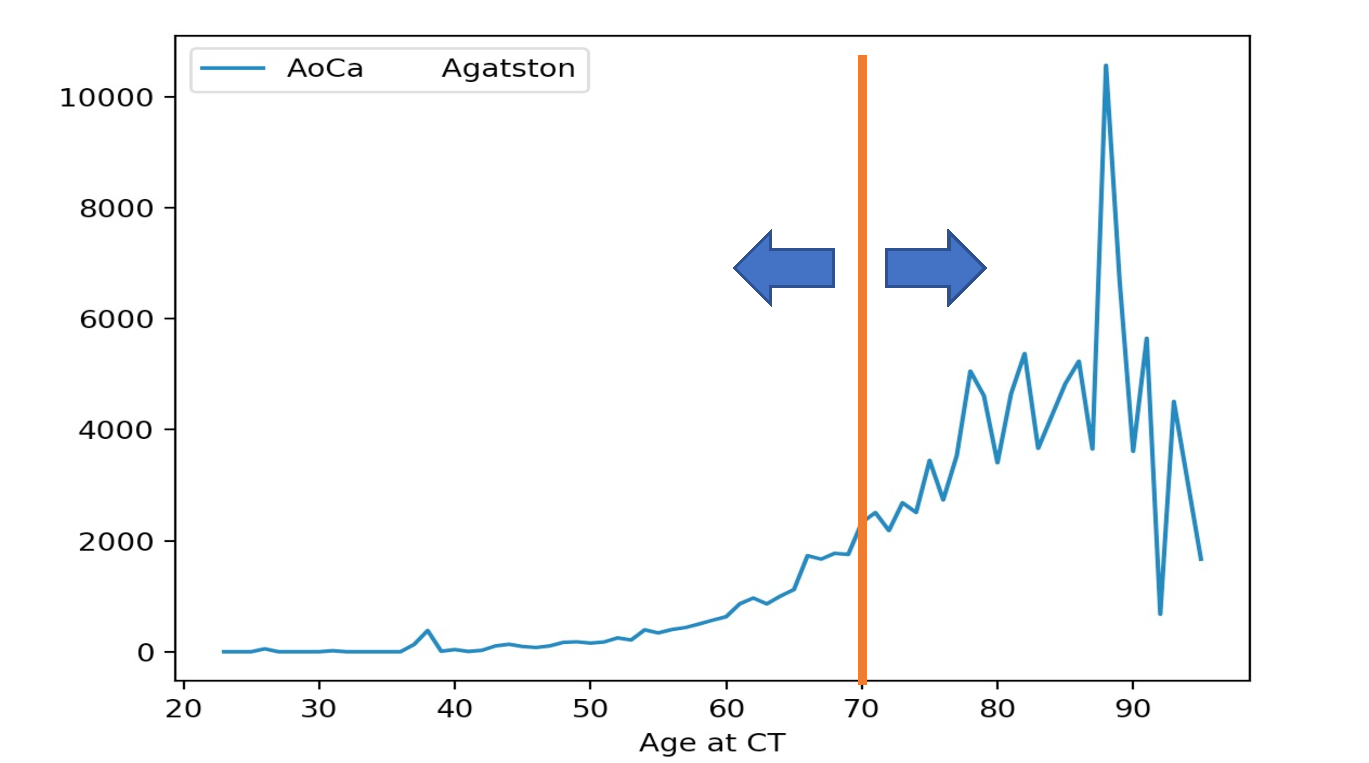
\includegraphics[width=0.65\textwidth]{figures/discrepancy.pdf}
    \caption{Data discrepancy in age distribution}
    \label{fig:discrepancy}
\end{figure}

\subsubsection{Classification and Regressions}
%그림 자리
We further analyze the data based on the distribution of age, and found out there is discrepancy between different ages, as shown in Figure~\ref{fig:discrepancy}.
That is, the value of AoCA Agaston increases in proportion to Age at CT within 70, but the observed values after then fluctuate, creating an irregular pattern.

To minimize the effect of the discrepancy, we classify the data into two groups, young and old, and run regression for each group.
We study our classification results in Section~\ref{sec:classification}.
Table~\ref{tab:clinical} reports the performance improvements between the previous and current increment.
Not only the accuracy with dead test data increases, but also that with alive test data improves by a large margin.

%We analyzed the data to improve the accuracy of the model and found that relation between age and CT data can be more explained, when we divide age into several groups. For example, in the case of AoCa Agaston, it increased in proportion to age until age 70, but had an irregular pattern from age 75. Furthermore, our classification model can distinguish someone is more than 70 or not with 85\% accuracy. So, if we divide the old and young groups using CT data and apply each regression model, we can have much higher accuracy. In fact, the accuracy improved by 15\% on average for each model.


\begin{table}[!h]
    \centering
    \caption{Prediction accuracy of classifications}
    \begin{tabular}{l||c|c|c}
        \toprule[0.8pt]
         \textbf{Models} & \textbf{Test with dead} & \textbf{Test with alive} & \textbf{50\% mixed} \\\hline
         Classification             & 16.22\% & 93.69\% & 54.96\% \\
         Balanced training data  & 64.83\% & 84.23\% & 74.53\% \\
         Augmented data          & 65.48\% & 85.81\% & 75.65\%\\
        \bottomrule[0.8pt]
    \end{tabular}
    \label{tab:classification}
\end{table}


\subsubsection{Classification}
\label{sec:classification}
We apply the same approach for classification as regressions stated above.
Table~\ref{tab:classification} shows the performance of stand-alone classification, classification with balanced training data, and augmented data (synthetically replicating dead data).
It follows the same performance trend as observed in the Section~\ref{sec:model_ct}.
Balanced ratio of the dead and alive data improves the accuracy for dead test data, and data augmentation further increases the performance of both tests.
We note that we use KNeighborsClassifier (KNN), GaussianNB (Naive Bayes), SGDClassifier (SVM), and MLPClassifier (Neural Network) in scikit-learn as our classifier models, but we only provide the results with MLPClassifier as using different classifiers only has small impact on the accuracy.
%We proceeded with the above- mentioned methods to improve the classification model of over 70 years or not. In addition, we proceeded data augment method. By adding over 80 years of age people more with simple transformation into the case of older group, we can improve classification model accuracy (from 74\% to 76\%)


\begin{figure}[!h]
    \centering
    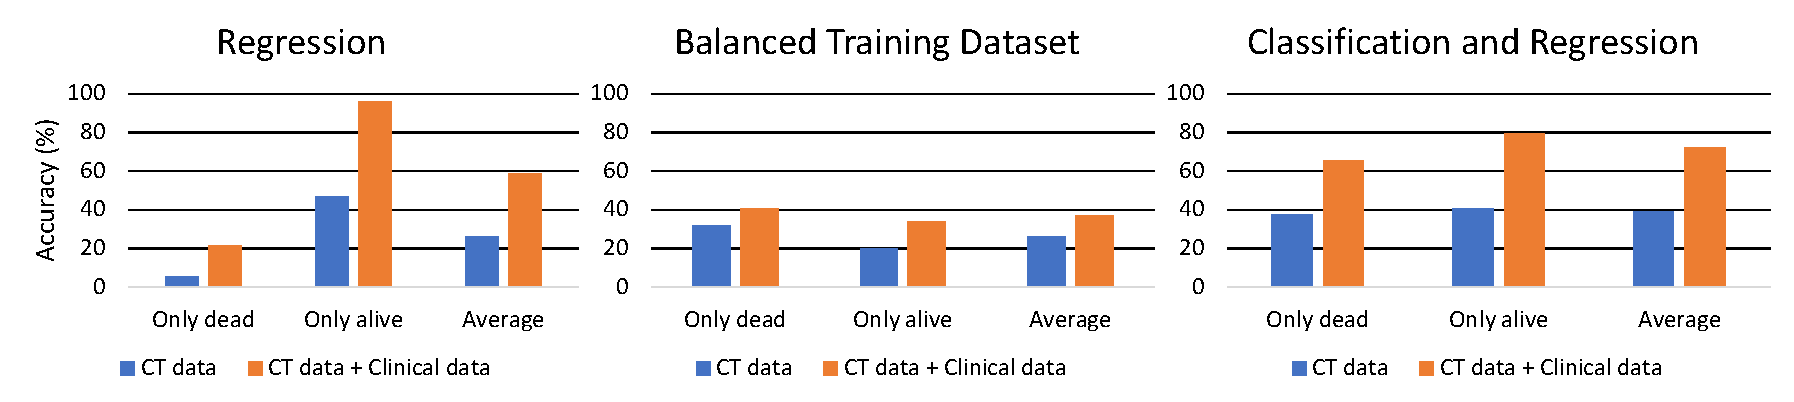
\includegraphics[width=0.95\textwidth]{figures/clinical.pdf}
    \caption{Accuracy comparisons with models using CT data, and models using both CT and clinical data}
    \label{fig:clinical}
\end{figure}

\subsection{Model Extension: using both Clinical and CT data}
\label{sec:clinical_CT}

We now apply our modeling approaches to further analyze the performance impact when clinical data are given.
Figure~\ref{fig:clinical} shows the accuracy comparisons between the models that use CT data, and the models that use both CT and clinical data for each approach.
The performance of those models using both CT and clinical data dominate that using CT data in every test case.

\begin{figure}[!h]
    \centering
    \begin{subfigure}{.48\textwidth}
        \centering
        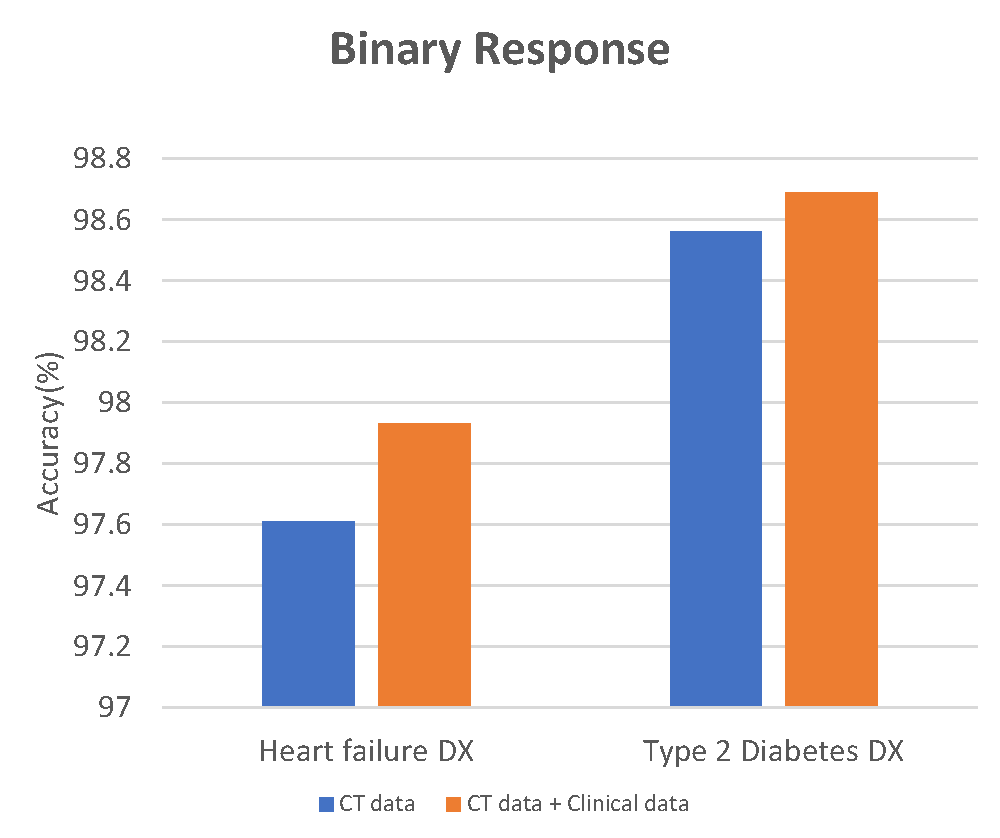
\includegraphics[width=.9\textwidth]{figures/binary_graph.pdf}
        \caption{Binary response}
        \label{fig:binary_outcome}
    \end{subfigure}
    \begin{subfigure}{.48\textwidth}
        \centering
        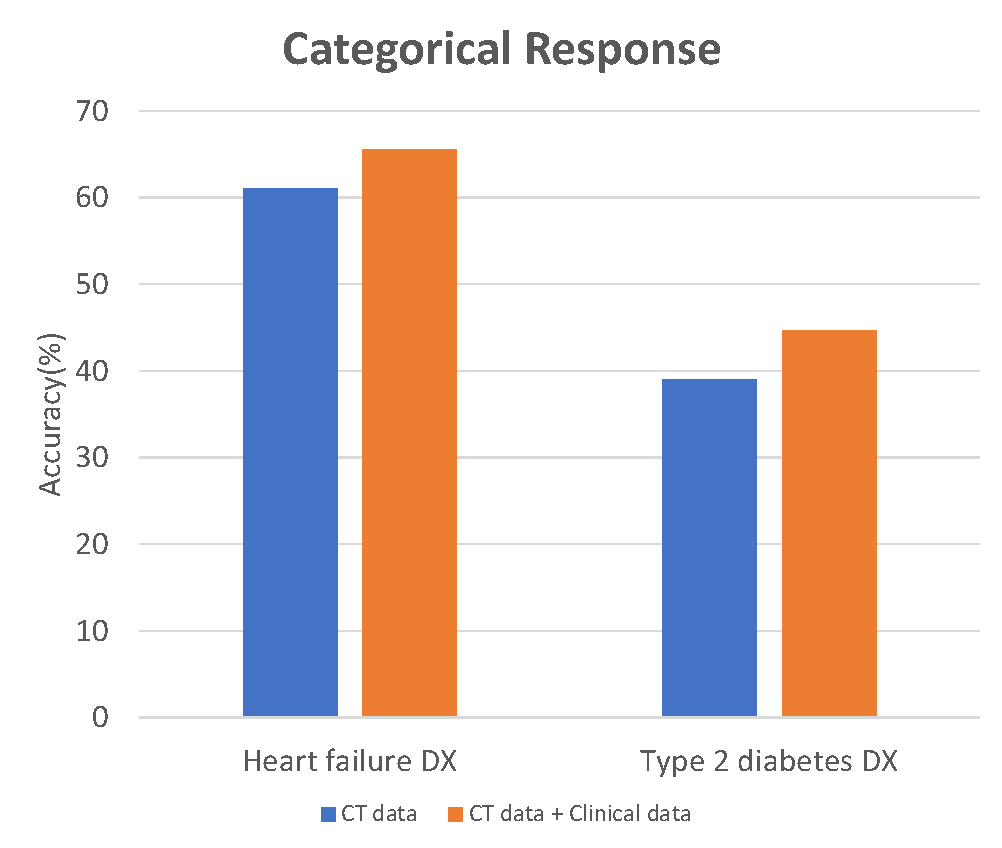
\includegraphics[width=.9\textwidth]{figures/categorical_graph.pdf}
        \caption{Categorical response}
        \label{fig:categorical_outcome}
    \end{subfigure}
    \caption{Accuracy comparisons with models using CT data, and models using both CT and clinical data for Heart Failure DX and Type 2 Diabetes DX prediction}
    \label{fig:clinical_outcome}
\end{figure}

\subsection{Model Extension: additional clinical outcomes}

Now we further dive into predicting additional clinical outcomes other than Death $[$d from CT$]$.
We use KNeighborsRegressor to predict a binary response, and a categorical response for Heart Failure DX and Type 2 Diabetes, as shown in Figure~\ref{fig:clinical_outcome}(a) and (b), respectively.
We note that the accuracy in each Figure is in a relative values, not fixing the range from 0 to 100\%.
From the results, we can infer that both the two models can efficiently predict Heart Failure DX and Type 2 Diabetes DX.
It is noteworthy that the accuracy improvement from the model using CT data to the model using both CT and clinical data is not as large as that observed in Section~\ref{sec:clinical_CT}.

%We predict Heart failure, Diabetes as additional clinical outcomes. KNN-regression(neighbor =10) has the best performance for this prediction and the detailed results are shown in the table below. The case using both CT data and clinical data shows 2.62\%(76.69\%,74.07\%) higher accuracy than the case where using only CT data. Especially,  when we predict 10 types of diabetes-DX messages and 27 types of heart failure-DX messages, using additional clinical data has a 5\% higher accuracy.

 %: x/y/prediction model 설명(step 1, 2, 3(problem + solution))/accuracy 측정 방법/prediction model 결과
\section{Biological Age}
\label{sec:bio}
In this section, we define our biological age, introduce its observation, and verify the biological age using the definition and observation. We define $AGE$ as the random variable for age and $BAGE$ as the random variable for our biological age. We also define $EXP$ as the random variable for life expectancy, which can be obtained by dividing predicted Death $[$d from CT$]$ by $365$.

\subsection{Definition and Observation}
We define $BAGE$ as follows:
\begin{definition}
$BAGE = AGE + \mathbb{E}\left(EXP | AGE\right) - EXP.$
\end{definition}
A person's $BAGE$ is same as the person's age under the assumption that the person will die when the person's age is $AGE + \mathbb{E}\left(EXP | AGE\right)$. As we will prove, $\mathbb{E}\left(BAGE | AGE\right) = AGE$. From this fact, we observe that $BAGE$ of a person with average CT data of healthy people with age $a$ is $a$.

\subsection{Verification Using Definition}
We define $X$ as $BAGE - AGE$, $\sigma$ as the standard deviation of $X$, which is unknown, $N$ as the number of our data, which is $8877$, $\bar{X}$ as the sample mean of $X$ for $N$ data, and $\hat{\bar{X}}$ as the mean of $X$ for our data. By the definition of $BAGE$, $X = \mathbb{E}\left(EXP | AGE\right) - EXP$. Taking mean on people with age $AGE$, we can get the following equality:
\begin{align*}
\mathbb{E}\left(X | AGE\right) &= \mathbb{E}\left(EXP | AGE\right) - \mathbb{E}\left(EXP | AGE\right)\\
&= 0.
\end{align*}
By central limit theorem, we can get the following information on the distribution of $\bar{X}$:
$$
\bar{X} \xrightarrow[]{d} \mathcal{N}\left(0, \frac{\sigma^2}{N}\right).
$$
To determine whether our biological age is valid, we define the following two hypotheses and select one hypothesis between the two:
%decide one hypothesis between those hypotheses:
\begin{gather*}
H_0: \hat{\bar{X}} \sim \mathcal{N}\left(\mu, \frac{\sigma^2}{N}\right), \mu = 0,\\
H_1: \hat{\bar{X}} \sim \mathcal{N}\left(\mu, \frac{\sigma^2}{N}\right), \mu \ne 0.
\end{gather*}
We use the following generalized likelihood ratio test where $\Phi_\chi$ is the tail function of $\chi^2$ distribution:
\begin{gather*}
\frac{\max\left\{\mathbb{P}\left(\hat{\bar{X}} | \mu\right): \mu \ne 0\right\}}{\mathbb{P}\left(\hat{\bar{X}} | \mu = 0\right)} \underset{H_0}{\overset{H_1}{\gtrless}} e^{\frac{1}{2} \Phi_\chi^{-1}\left(0.05\right)}.
\end{gather*}
Computing the left hand side of the above inequality, we can rewrite the test as follows:
\begin{gather*}
\left(\frac{\hat{\bar{X}}}{\frac{\sigma}{\sqrt{N}}}\right)^2 \underset{H_0}{\overset{H_1}{\gtrless}} \Phi_\chi^{-1}\left(0.05\right).
\end{gather*}
$\hat{\bar{X}} = 57.41 - 56.91 = 0.5$, and $N = 8877$. Hence, $\left(\frac{\hat{\bar{X}}}{\frac{\sigma}{\sqrt{N}}}\right)^2 \le \Phi_\chi^{-1}\left(0.05\right)$ if and only if $\sigma \ge 24.04$. Considering the definition for $X$, $24.04$ is relatively high value as $\sigma$, but it is reasonable that $\sigma = 24.04$, so we conclude that our biological age is fairly valid using the definition for our biological age.

\subsection{Verification Using Observation}
As we create models predicting clinical outcome using CT data, we can also create models predicting biological age using CT data. Based on the observation for our biological age, we guess that predicted biological age of a person with average CT data of healthy people with age $a$ is near to $a$. For this reason, we also verify our biological age using the models predicting biological age using CT data.

We create 2 models predicting biological age using CT data using the methodology of the models predicting clinical outcome using CT data. The first model is the model predicting biological age using regression. The second model is the model classifying data as data in old group and data in young group and predicting biological age using regression for each group. We use KNeighborsRegressor, MLPRegressor, and GaussianNB in scikit-learn as our regressors. Biological age can be considered as discrete variable, so we use GaussianNB as one of regressors. We use KNeighborsClassifier, MLPClassifier, and GaussianNB in scikit-learn as our classifiers. We only provide the results for KNeighborsClassifier because classifiers have almost no effect on the accuracy of the models.

We use all the tuples in CT data for training our models. The test data are the average CT data of healthy people with age $a$ for all $a$. We define a healthy person as a person who is predicted to live after 3 years, so we exclude data who are predicted to die in 3 years when we make test data. We consider prediction is correct if the difference of predicted biological age and age is not bigger than 3 years. We believe that predicting precise biological age is as hard as predicting precise death dates, and if the models are correct, and our biological age is valid, predicted biological age is near from age for test data, so we define correct prediction in this way.

Table~\ref{tab:bio} shows the prediction accuracy of the models for the case that regressor is KNeighborsRegressor, MLPRegressor, and GaussianNB, and classifier is KNeighborsClassifier. Accuracy of the second model is higher than that of the first model, accuracy of the model with GaussianNB regressor is higher than that of the models with the other regressors, and the highest accuracy is attained as 63.64\%. This accuracy is fairly high, so we conclude that our biological age is fairly valid using the observation for our biological age.

\begin{table}[!h]
    \centering
    \caption{Accuracy of models predicting biological age}
    \begin{tabular}{l||c|c|c}
        \toprule[0.8pt]
         \textbf{Models} & \textbf{KNN regression} & \textbf{Neural network} & \textbf{Gaussian naive Bayes}\\\hline
         Regression & 27.27\% & 25.45\% & 50.91\%\\
         Classification and regression & 30.91\% & 29.09\% & 63.64\%\\
        \bottomrule[0.8pt]
    \end{tabular}
    \label{tab:bio}
\end{table}
\section{Conclusion}
\label{sec:conclusion}

In this work, we predict clinical outcomes using CT data and clinical data.
We utilize different machine learning models from classifiers and regressors.
Based on our extensive data analysis, we present three modeling approaches, regression, regression with balanced training data, and classification and regression with balanced training data.
Our evaluation study shows each incremental brings huge performance gain.
We further extend our models to predict additional clinical outcomes such as diabetes and heart failure.
We define our biological age based on an individual's chronological age, average life expectancy and predicted life expectancy.
Our verification with definition and modeling observation concludes that the biological age is valid.

In the future, we want to improve models using more training data. If we have more training data of young people, we can classify data into more than 2 groups, so regression for each group will be improved. Also, if we have more training data of dead people, more real data will be used as training data, so models become more realistic.

\bibliographystyle{abbrvurl}
\bibliography{bib.bib}

\end{document}